\documentclass[11pt,a4paper]{report}

\evensidemargin=0cm
\oddsidemargin=0cm
\topmargin=-1cm
\textheight=23.5cm
\leftmargin=0cm
\textwidth=18cm
\sloppy
\flushbottom
\parindent 1em
\hoffset -0.5in
\oddsidemargin  0pt
\evensidemargin 0pt
\marginparsep 10pt

\usepackage[utf8]{inputenc}
\usepackage[frenchb]{babel}
\usepackage[T1]{fontenc}

\usepackage{graphicx}

\usepackage{listings}
\usepackage{color}
\definecolor{lightgray}{rgb}{.9,.9,.9}
\definecolor{darkgray}{rgb}{.4,.4,.4}
\definecolor{purple}{rgb}{0.65, 0.12, 0.82}

\lstnewenvironment{OCaml}
                  {\lstset{
                      language=[Objective]Caml,
                      breaklines=true,
                      commentstyle=\color{purple},
                      stringstyle=\color{red},
                      identifierstyle=\ttfamily,
                      keywordstyle=\color{blue},
                      basicstyle=\footnotesize
                    }  
                  }
                  {}
\lstnewenvironment{C}
                  {\lstset{
                      language=C,
                      breaklines=true,
                      commentstyle=\color{purple},
                      stringstyle=\color{red},
                      identifierstyle=\ttfamily,
                      keywordstyle=\color{blue},
                      basicstyle=\footnotesize
                    }  
                  }
                  {}

\title{Rapport de projet\\Débogueur Visuel pour OCaml}
\author{Mathieu Chailloux\\Vincent Botbol}
\date\today

\begin{document}
\maketitle

\chapter{Introduction}

Bien que le langage OCaml soit considéré comme un langage sûr de par la sécurité de son typage statique et fort, % trouver +
l'utilisateur n'est pas à l'abri de problèmes algorithmique ou ... . La distribution de base du langage inclut %todo
un débogueur, \emph{ocamldebug}, en ligne de commande. Cependant, son utilisation est parfois mal adaptée au besoin du programmeur.

Notre projet tente de répondre à ces problèmes en apportant au débogueur une interface graphique simple ainsi quelques
outils supplémentaires facilitant l'emploi du logiciel. Nous nous approchons d'outils similaires
tel que \emph{ddd} pour \emph{gdb}, l'interface graphique du célèbre débogueur pour le langage C. Notre logiciel se concentre
principalement sur l'aspect ergonomique d'un  bien qu'une grande partie de notre travail visa à améliorer certains
aspects du débogueur déjà présent.
% ^ tourner ça plus correctement

Pour expliciter les forces et les faiblesses d'\emph{ocamldebug}, nous détaillerons, dans une première partie:
l'utilisation de cet outil et son fonctionnement interne.

Nous présenterons ensuite notre outil, les extensions développées et certaines de ses possibilités d'améliorations.

\chapter{Ocamldebug}

\section{Présentation}

\emph{Ocamldebug} est le débogueur officiel d'OCaml. Cet outil permet à l'utilisateur d'avancer au fur et à mesure
dans l'exécution de son programme grâce à un système d'\emph{événements d'exécution}. Il dispose aussi de
fonctionnalités de ``retour arrière'' dans l'exécution. Son interface est en ligne de commande bien qu'un mode existe 
pour s'exécuter avec l'éditeur de texte \emph{Emacs} permettant une visualisation de l'état du programme.

%il établit une connexion avec la vm
Au démarrage, le débogueur établit une connexion avec la machine virtuelle via un connecteur réseau.

%todo

%topo
%exemple d'utilisation
%liste des commandes

\section{\'Evénements de débogage}

Nous allons détailler dans cette partie les actions effectuées par le compilateur qui vont servir à ocamldebug. Pour le lecteur curieux, sachez que les fichiers que nous allons citer se situe dans le dossier ``bytecomp'' (composition du bytecode) de la distribution ``OCaml''.

\subsection{Capture des informations de compilation}

Il est possible lors de la compilation, par l'option ``-g'' d'ocamlc (OCaml compiler), de stocker des informations sur l'environnement en cours. Ces informations sont considérées comme des événements (debug\_event, cf instruct.ml) qui contiennent de précieuses données comme l'environnement de compilation (plus précisément, la place de chaque variable), la taille de pile, le module courant ou encore la position de l'expression correspondante (en train d'être compilée) dans le code source. Cette dernière information permet donc une meilleure lisibilité du débogueur (le lien entre instruction bytecode et programme source étant du coup immédiate). Voici le type de ces événements :

\begin{OCaml}

type debug_event =
  { mutable ev_pos: int;                (* Position in bytecode *)
    ev_module: string;                  (* Name of defining module *)
    ev_loc: Location.t;                 (* Location in source file *)
    ev_kind: debug_event_kind;          (* Before/after event *)
    ev_info: debug_event_info;          (* Extra information *)
    ev_typenv: Env.summary;             (* Typing environment *)
    ev_typsubst: Subst.t;               (* Substitution over types *)
    ev_compenv: compilation_env;        (* Compilation environment *)
    ev_stacksize: int;                  (* Size of stack frame *)
    ev_repr: debug_event_repr }         (* Position of the representative *)

\end{OCaml}

\medskip

\subsection{Construction des événements}

Comme évoqué à l'instant, ces évènements sont construits à partir des expressions à compiler, en fait plus précisément à partir de l'AST typé (type\_expr), et sont produits en 3 étapes :

\medskip

\begin{itemize}

\item Lors de la transformation (cf translcore.ml) de l'arbre de syntaxe abstrait (AST) typé en lambda-termes (lambda.ml) (???A COMPRENDRE???). Ce premier niveau permet de conserver la localisation avec le source, l'environnement de types, ainsi que le type de l'évènement, nous reviendrons sur ce dernier point plus tard. Le lambda-terme normalement obtenu est alors enveloppé dans un autre lambda-terme (Levent) qui contient ces informations.

\item Lors de la production des instructions bytecode (bytegen.ml), ce qui permet alors de vraiment capturer l'environnement de compilation, par le biais d'une instruction Kevent.

\item Enfin, lors de l'émission effective du bytecode (emitcode.ml), lorsqu'une instruction Kevent est rencontrée, l'évènement (auquel on ajoute le pc auquel il devrait se trouver) qu'elle porte est stocké dans une liste d'évènement qui est ensuite écrite à la suite du bytecode dans le fichier.

\end{itemize}

\medskip

\subsection{Représentation des événements}

Nous avons évoqué plus haut le type des évènements. On ne parle pas ici de type au sens d'un langage de programmation mais plus de représentation. En, effet, on a vu qu'ils sont produits à partir des expressions de l'AST. Ils peuvent alors contenir des informations sur ces dernières, ou encore sur d'autre événements :

\begin{OCaml}

and debug_event_kind =
    Event_before
  | Event_after of Types.type_expr
  | Event_pseudo

and debug_event_info =
    Event_function
  | Event_return of int
  | Event_other

and debug_event_repr =
    Event_none
  | Event_parent of int ref
  | Event_child of int ref

\end{OCaml}

Le premier type somme correspond à la position de l'événement par rapport à l'expression (cela nous permet notament de retrouver sa localisation dans le source, qui est celle de début ou de fin de l'expression auquel il se réfère). Le dernier constructeur indique s'il est virtuel (par exemple lors de la compilation d'un mot-clé ``function'', on place un événement virtuel au début, quelle que soit la branche effectivement empruntée).

\smallskip

Le second type somme permet juste de conserver les cas particuliers des fonctions, et des retours (qui sont en fait des événements ``Event\_after'' d'un appel de fonction ou de méthode). L'entier associé capture l'arité de la fonction ou la méthode.

\smallskip

Enfin, le troisième type permet de représenter les relations qu'il peut y avoir entre événements. TODO




\bigskip

Ainsi, lors du chargement du programme à déboguer, il est possible de récupérer la liste des événements. Il s'agit maintenant de découvrir comment ils sont exploités pour permettre une correcte exécution du programme tout en profitant des fonctionnalités d'un débogueur.

\section{Communication avec la machine virtuelle}

Comme évoqué, ocamldebug communique avec la VM, il a donc été essentiel pour nous de comprendre comment ces deux programmes pouvait collaborer de façon cohérente. Une fois les événements chargés, le débogueur et la VM vont communiquer à travers une socket (une interface de connexion pour les puristes). Ces échanges vont suivre le modèle client/serveur où ``ocamldebug'' envoie des requêtes à la VM qui peuvent modifier son état et éventuellement attendent une réponse.


\medskip

\subsection{Chargement des événements}

Lors du lancement d'ocamldebug, les événements sont lus et stockés dans des tables de hachages (cf debugger/symbols.ml) par module et par compteur de programme (que l'on nommera ``pc'' par la suite). Puis, le débogueur communique à la VM tous les événements accompagnés de leur pc. La stratégie alors utilisée s'appuie sur l'usage de deux nouvelles instructions bytecode : ``EVENT'' et ``BREAK''
qui ne sont jamais émises par le compilateur. La VM est alors en mesure, grâce au pc, de remplacer les anciennes instructions par ``EVENT'', ainsi on peut effectuer un traitement spécifique lorsque l'exécution arrive sur une telle instruction. Il faut aussi enregistrer le programme initial, sans ``EVENT'', afin de pouvoir garder une exécution correcte, mais nous détaillerons ce point plus tard. Nous allons maintenant nous intéresser à la façon dont ``ocamldebug'' envoie ses requête à la VM.

\medskip

\subsection{Requêtes ocamldebug -> VM}

Nous venons de voir qu'il était possible de placer des événements dans le code exécuté mais le protocole établi entre ocamldebug et la VM permet de nombreuses manipulations. En effet, on peut donc placer un événement, un breakpoint (un événement sur lequel la VM s'arrête forcément), ou encore les retirer du code exécuté. Une fonctionnalité bien utile est l'accès aux variables, quelles qu'elles soient (sur la pile, dans le tas, globales), notament grâce à la position dans leur environnement que l'on a enregistré au moment de la compilation. Il est encore possible d'accéder à la valeur de l'accumulateur, de modifier le pointeur de pile ou d'y accéder, de lancer l'exécution, de l'arrêter, ...

\smallskip

Ci-après vient la liste des requêtes du protocole telle que décrites dans ``byterun/debugger.h'' :

\medskip

\begin{C}

enum debugger_request {
  REQ_SET_EVENT = 'e',          /* uint32 pos */
  /* Set an event on the instruction at position pos */
  REQ_SET_BREAKPOINT = 'B',     /* uint32 pos, (char k) */
  /* Set a breakpoint at position pos */
  /* In profiling mode, the breakpoint kind is set to k */
  REQ_RESET_INSTR = 'i',        /* uint32 pos */
  /* Clear an event or breapoint at position pos, restores initial instr. */
  REQ_CHECKPOINT = 'c',         /* no args */
  /* Checkpoint the runtime system by forking a child process.
     Reply is pid of child process or -1 if checkpoint failed. */
  REQ_GO = 'g',                 /* uint32 n */
  /* Run the program for n events.
     Reply is one of debugger_reply described below. */
  REQ_STOP = 's',               /* no args */
  /* Terminate the runtime system */
  REQ_WAIT = 'w',               /* no args */
  /* Reap one dead child (a discarded checkpoint). */
  REQ_INITIAL_FRAME = '0',      /* no args */
  /* Set current frame to bottom frame (the one currently executing).
     Reply is stack offset and current pc. */
  REQ_GET_FRAME = 'f',          /* no args */
  /* Return current frame location (stack offset + current pc). */
  REQ_SET_FRAME = 'S',          /* uint32 stack_offset */
  /* Set current frame to given stack offset. No reply. */
  REQ_UP_FRAME = 'U',           /* uint32 n */
  /* Move one frame up. Argument n is size of current frame (in words).
     Reply is stack offset and current pc, or -1 if top of stack reached. */
  REQ_SET_TRAP_BARRIER = 'b',   /* uint32 offset */
  /* Set the trap barrier at the given offset. */
  REQ_GET_LOCAL = 'L',          /* uint32 slot_number */
  /* Return the local variable at the given slot in the current frame.
     Reply is one value. */
  REQ_GET_ENVIRONMENT = 'E',    /* uint32 slot_number */
  /* Return the local variable at the given slot in the heap environment
     of the current frame. Reply is one value. */
  REQ_GET_GLOBAL = 'G',         /* uint32 global_number */
  /* Return the specified global variable. Reply is one value. */
  REQ_GET_ACCU = 'A',           /* no args */
  /* Return the current contents of the accumulator. Reply is one value. */
  REQ_GET_HEADER = 'H',         /* mlvalue v */
  /* As REQ_GET_OBJ, but sends only the header. */
  REQ_GET_FIELD = 'F',          /* mlvalue v, uint32 fieldnum */
  /* As REQ_GET_OBJ, but sends only one field. */
  REQ_MARSHAL_OBJ = 'M',        /* mlvalue v */
  /* Send a copy of the data structure rooted at v, using the same
     format as [caml_output_value]. */
  REQ_GET_CLOSURE_CODE = 'C',   /* mlvalue v */
  /* Send the code address of the given closure.
     Reply is one uint32. */
  REQ_SET_FORK_MODE = 'K'       /* uint32 m */
  /* Set whether to follow the child (m=0) or the parent on fork. */
};

\end{C}

\medskip

\subsection{Gestion des requêtes}

Nous allons maintenant nous intéresser à la façon dont la VM traite ces requêtes (fonction ``caml\_debugger'' du fichier ``byterun/debugger.c''). De base, la VM est en attente sur la socket (lecture bloquante) de requêtes. Dès qu'elle en reçoit une, elle effectue le traitement approprié (placement d'un événement par exemple), envoie une réponse si nécessaire (accès à une valeur par exemple), et boucle ainsi sur la lecture de requête. Dans un seul cas il est possible de sortir de cette boucle, c'est lors d'une requête d'exécution (``REQ\_GO''), quel que soit le pas associé. C'est alors la VM qui effectue une exécution traditionnelle jusqu'à rencontrer une raison de s'arrêter :

\smallskip

\begin{itemize}
\item On a effectué le nombre de pas demandé. Par exemple si on veut avancer de 5 événements, la VM s'arrête une fois la cinquième instruction ``EVENT'' rencontrée.
\item On rencontre un breakpoint, représenté par l'instruction ``BREAK''.
\item L'exécution du programme est finie.
\item La limite de la pile (que l'on peut fixer par une requête) a été atteinte.
\item Le programme se termine à cause d'une exception non rattrapée.
\end{itemize}

\smallskip

La VM envoie alors la raison de son interruption. De plus, si celle-ci est dûe à un événement ou un breakpoint, alors on envoie aussi les nouveaux pointeur de pile et pc.

\smallskip

Voici le type qui représente ces réponses :

\smallskip

\begin{C}

enum debugger_reply {
  REP_EVENT = 'e',
  /* Event counter reached 0. */
  REP_BREAKPOINT = 'b',
  /* Breakpoint hit. */
  REP_EXITED = 'x',
  /* Program exited by calling exit or reaching the end of the source. */
  REP_TRAP = 's',
  /* Trap barrier crossed. */
  REP_UNCAUGHT_EXC = 'u'
  /* Program exited due to a stray exception. */
};

\end{C}

\smallskip

Enfin, lorsqu'une nouvelle demande d'exécution est reçue et que l'on s'était arrêté sur un événement ou un breakpoint, alors la VM recommence son exécution au même pc, en remplaçant l'instruction de débogage par la véritable instruction du code initial (qui avait été sauvegardé comme évoqué précédemment et que l'on retrouve grâce au pc).


\section{Limitations et inconvénients} % transition


\chapter{OCabug}

%intro : ce qu'on a fait
%présentation des différentes extensions, installation, ocaml 3.12...
%patch du compilo


\section{Présentation de l'interface}

L'interface graphique de l'application a entièrement été réalisée avec LablGtk, le ``binding'' de Gtk pour OCaml.
Elle assure un confort visuel à l'utilisateur en permettant un accès rapide aux commandes les plus utilisées ainsi
que l'observation directe des différents fichiers sources permettant de constater la position courante 
et des différents ``breakpoints'' du programme. Le toplevel d'ocamldebug est également présent pour afficher
les différentes actions du débogueur et les sorties textuelles engendrées.

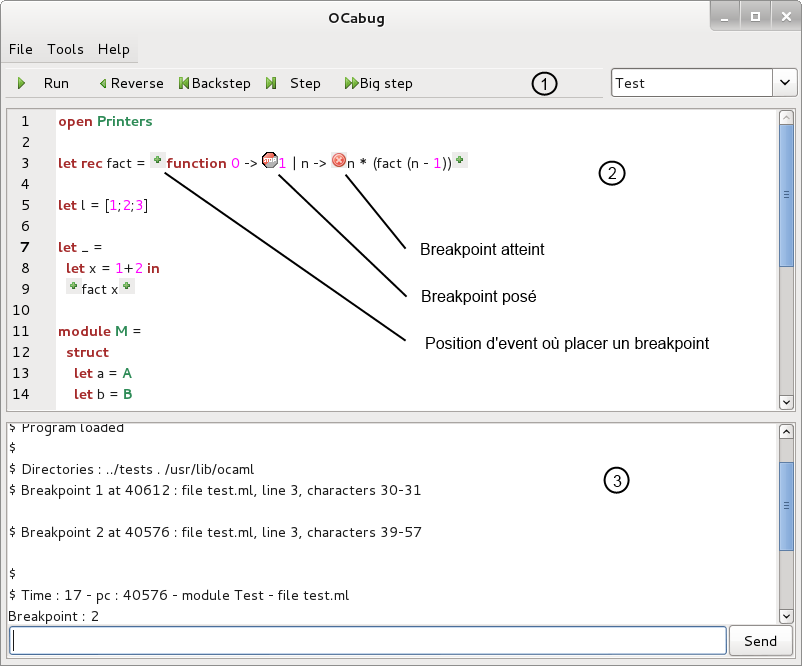
\includegraphics{screen_exec}

\begin{enumerate}
\item Barre d'outils et séléction du module à afficher
\item Affichage du fichier source du module courrant enrichi des événements de débogage activables
\item Informations textuelles et invite de commande
\end{enumerate}

L'utilisateur a activé deux ``breakpoints'' en cliquant sur les ``+'' présent dans l'affichage du source.
Il démarre ensuite le programme en appuyant sur \emph{Run} qui s'arrête au premier breakpoint rencontré,
changeant temporairement son icône ``Stop'' par un ``X'' rouge.

\subsection{Barre d'outils}

Les différents boutons incluent dans la barre d'outils réunissent les commandes les plus communes lors de l'utilisation:
\begin{itemize}
\item Run -- Permet de lancer le programme. Celui-ci s'arrêtera lorsqu'un breakpoint sera rencontré ou simplement à la fin du programme.
\item Reverse -- Action symétrique au Run; Parcours le programme en sens inverse toujours en s'arrêtant au breakpoint ou au début du programme.
\item Backstep -- Recule d'un événement de débogage.
\item Step -- Avance d'un événement de débogage
\item Big step -- Avance au prochain événement en omettant ceux de module différent.
\item Liste des modules -- Permet de basculer l'affichage des différents fichiers sources présents.
\end{itemize}

\subsection{Code source}

Le panneau du code source a d'autres emplois que la simple visualisation du programme. 
Il permet également à l'utilisateur de poser des breakpoints dans le code au niveau des événements du débogage.

Chaque icône a sa signification particulière:
\begin{itemize}
\item Symbole ``+'' vert -- \'Evénement de débogage: un click active la pose d'un breakpoint à cet endroit du code
\item Symbole ``+'' gris entouré -- Position actuelle du programme
\item Panneau ``Stop'' -- Breakpoint actif: un click le retire
\item Croix rouge -- Position actuelle du programme ayant atteint un breakpoint
\end{itemize}

\subsection{Toplevel}

La console affichant le toplevel permet à l'utilisateur de constater les différents affichages du programme
et du débugueur. Les commandes entrées par l'utilisateur dans la zone de saise sont interprétées de la même
manière que pour ``ocamldebug'' en supportant également nos propres commandes.

\section{Placement par rapport à Ocamldebug}

Notre implémentation se base sur le noyau d'``ocamldebug''. Nous avons repris le code originel et
avons adapter les mécanismes d'entrées/sorties console pour les convertir à une utilisation
graphique. Il nous a ensuite fallu lié les différents composants de l'interface aux fonctions du débogueur
tout en maintenant une cohérence entre les commandes entrées manuellement et l'utilisation de l'interface.
Nous maintenons ainsi toutes les fonctionnalités originelles du débogueur. 

La modification du noyau est restée nécessaire pour pouvoir nous permettre d'ajouter nos propres commandes.
...

%nécessite le compilo + lablgtk (ici?)
\section{Implémentation des extensions}

Nous avons principalement deux extensions à notre disposition.
Premièrement, la commande ``Big step''. A plusieurs moments, le programmeur ne
peut ne pas souhaiter se déplacer dans des modules externes lors d'un débogage.
Notre commande considère alors le module courant et passe au prochain événement
qu'il rencontrera dans ce même module.

Techniquement, cette commande agit de la même manière qu'un ``step'' en vérifiant 
en plus, à chaque avancement, que l'événement appartient bien au même module. 
Si ça n'est pas le cas, on continue jusqu'à ce que la condition soit satisfaite.

Nous disposons également d'une instruction de déplacement filtrant les modules
appartenant à la librairie standard. En effet, la plupart du temps, nous ne souhaitons
pas rentrer dans le code de la bibliothèque standard. Nous pouvons ainsi nous abstraire
des différentes fonctions que l'utilisateur considère comme sûres pour nous consacrer
exclusivement au code en cours de débogage. On peut noter aussi la présence d'une option
pour ajouter ou enlever des modules à la liste des filtres actifs. 

Pour implémenter un tel comportement, nous récupérons tout d'abord la liste des modules standards
d'OCaml grâce à la variable d'environnement contenant le chemin vers leur dossier. Nous pouvons ensuite
filtrer selon le module de l'événement atteint si celui-ci est éligible ou non.
% + ?

Ce comportement concerne le bouton ``step'' de l'interface et est activé par défaut. 
Ceci peut, à tout moment, être modifié via le menu de l'application.

\section{Améliorations possibles}
%threads
%compteur

\chapter{Conclusion}

%whine sur le bordel que c'était
%compréhension du débogueur
%adaptation d'ocamldebug

\chapter{Annexes}

\section{Exemples}
\section{Liste des commandes}

\end{document}
